% File name: ufem-cz.tex
% Date:      2009/10/28 12:34
% Author:    Jiri Brozovsky

% Cesky manual pro uFEM GUI - pro zacatecniky

\documentclass[12pt, a4paper, oneside]{book}
\usepackage{latexsym}
\usepackage{czech}
\usepackage{graphicx} % for .eps images
\usepackage{hyperref}
\usepackage{fancyhdr}

\title{ufem-cz}
\author{Ji\v{r}\'{\i} Bro\v{z}ovsk\'{y}}
\date{\today}

%\hyphenation{}

\voffset = -20 mm
\textheight = 240 mm
\hoffset = -8 mm
\textwidth = 152 mm
\footskip = 18 mm



%%%%%%%%%%%%%%%%%%%%%%%%%%%%%%%%%%%%%%%%%%%%%%%%%%%%%%%%%%%%%%%%%%
\begin{document}
\pagestyle{empty}
%toto je jako titulni list
\begin{center}
%\enlargethispage{240mm}
\renewcommand{\arraystretch}{1.3}
{\begin{tabular}{c} 
{\Large\textsc{Program uFEM}} \\
\hline
{\large{ ~~~ Vyu�it� metody kone�n�ch prvk� v mechanice kontinua ~~~ }}\\
\end{tabular}}

\vspace{64mm}
{\large ~~~}  \\
\vspace{6mm}
\section*{\Large \sc 
U�ivatelsk� p��ru�ka 
}
\vspace{16mm}
{\large  Ji\v{r}\'{\i} Bro\v{z}ovsk\'{y}}
\vfill
\scalebox{.2}{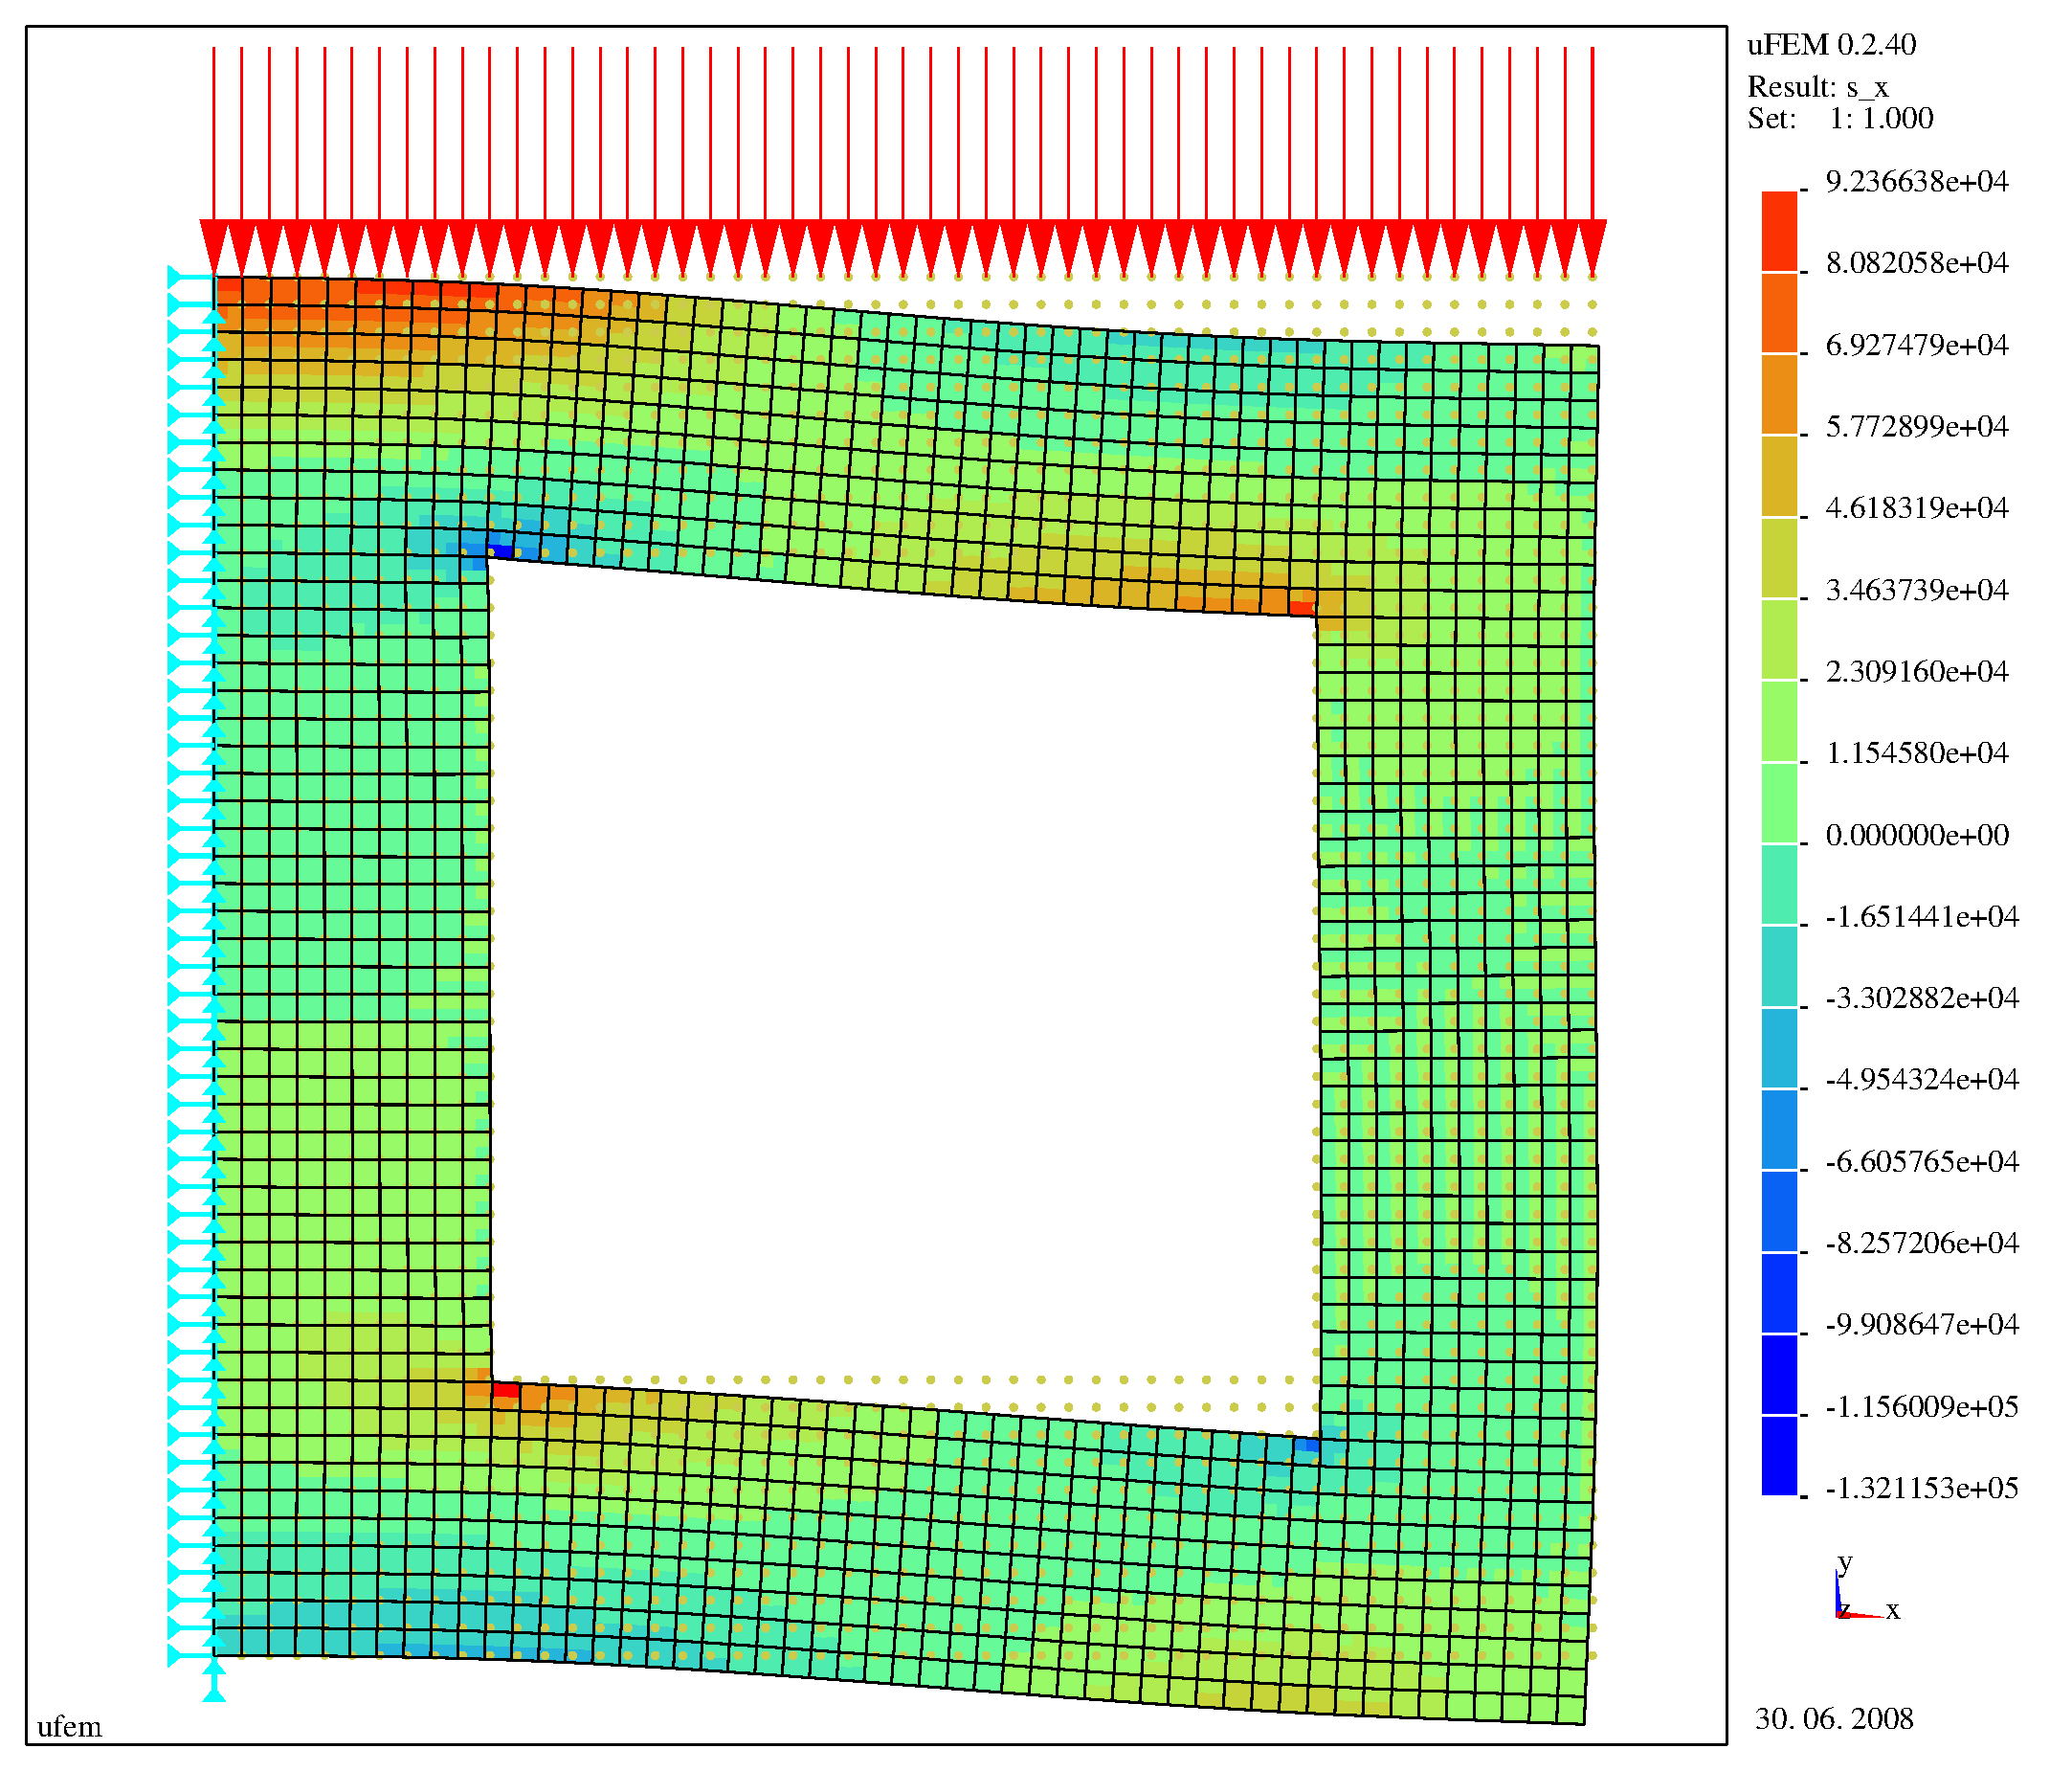
\includegraphics{ufem-plot.eps}}
\vfill
~\\
{\large Ostrava, \today}
\end{center}

\newpage

% -----------------------------------------------------------------------

% TADY TO VELEDILO ZACINA:


\frontmatter

\pagestyle{plain}

% obsah je velmi dulezity:
\tableofcontents
% taktez seznam obrazku (to kazdeho zajima nejvic ;-)
%\listoffigures
% a co teprve seznam tabulek
%\listoftables
% pouzite znaceni je take strasne dulezite:
%\input znacky

% anotace cesky a anglicky (1+1 str)
%--

\mainmatter

\fancypagestyle{plain}{                     % redefinice stylu plain
\fancyhf{}\fancyfoot[C]{\thepage}%
\renewcommand{\headrulewidth}{0pt}}
\pagestyle{fancy}
\rhead{}

\flushbottom

% uvod
\chapter{�vod}
\input u-cz-uvod

% prvni kroky
\chapter{Prvn� kroky v programu}
\input u-cz-1sh

% prvni kroky
\chapter{Operace v grafick�m prost�ed�}
\input u-cz-gfx

% prvni kroky
\chapter{Geometrick� model}
\input u-cz-geo

% prvni kroky
\chapter{Kone�n�prvkov� model}
\input u-cz-kp


% prvni kroky
\chapter{Spu�t�n� v�po�tu}
\input u-cz-sol

% prvni kroky
\chapter{Pr�ce s v�sledky}
\input u-cz-res

% prvni kroky
%\chapter{P��kazov� jazyk}
%\input u-cz-cmd

%% numericke priklady:
%\chapter{Numerick� p��klady}
%\input numpr

% instalace
\chapter{Instalace programu}
\input u-cz-inst

% seznam literatury:
\input u-lit-cz
%--


\end{document}
%%%%%%%%%%%%%%%%%%%%%%%%%%%%%%%%%%%%%%%%%%%%%%%%%%%%%%%%%%%%%%%%%%
